\documentclass{beamer}

\usepackage{graphics}
\usepackage{graphicx}
\usepackage{amsmath,amssymb,amsthm}
%\usepackage{subeqnarray}
%\usepackage{easybmat}
%\usepackage{subfigure}



%\usepackage{HA-prosper}
%\usepackage[dvips,letterpaper]{geometry}

\def\Proba#1{\mathcal{P}\left(#1\right)}
\def\Surv{\mathcal{S}}
\def\R{\mathcal{R}}
\def\D{\mathcal{D}}
\def\C{\mathcal{C}}
\def\IC{\mathbb{C}}
\def\IN{\mathbb{N}}
\def\IR{\mathbb{R}}
\def\IZ{\mathbb{Z}}
\def\Rzero{\mathcal{R}_0}
\def\diag{\textrm{diag}}
\def\tr{\textrm{tr}}
\def\det{\textrm{det}}
\def\sgn{\textrm{sgn}}
\def\imply{$\Rightarrow$}
\def\dbint{\int\!\!\!\int}
\def\dbintb{\mathop{\int\!\!\!\!\int}}
\def\tpint{\int\!\!\!\int\!\!\!\int}

\def\red{\color[rgb]{1,0,0}}

\newtheorem{proposition}{Proposition}

\setbeamertemplate{navigation symbols}{}
\setbeamertemplate{footline}
{%
\quad\insertsection\hfill p. \insertpagenumber\quad\mbox{}\vskip2pt
}

\title[Epidemic models]{A few epidemic models\vskip1cm Introduction to the analysis of nonlinear systems of ordinary differential equations}
\date{}

\begin{document}
\frame[plain]{\setcounter{page}{0}\titlepage}
%%%%%%%%%%%%%%
%%%%%%%%%%%%%%


\section{SIS model without vital dynamics}
\frame[plain]{\tableofcontents[current]}
%\frame[plain]{\addtocounter{page}{-1}\tableofcontents[current]}


\frame{\frametitle{A SIS model}
Consider a disease that confers no immunity. In this case,
individuals are either
\begin{itemize}
\item \emph{susceptible} to the disease, with the number of such individuals at time $t$ denoted by $S(t)$,
\item or \emph{infected} by the disease (and are also \emph{infective} in the sense that they propagate the disease), with the number of such individuals at time $t$ denoted by $I(t)$.
\end{itemize}
\vskip1cm
We want to model the evolution with time of $S$ and $I$ ($t$ is omitted unless necessary).
}

\frame{\frametitle{Hypotheses}
\begin{itemize}
\item Individuals recover from the disease at the \emph{per capita} rate $\gamma$.
\item The disease does not confer immunity.
\item There is no birth or death.
\item Infection is of \emph{standard incidence} type, $\beta=SI/N$.
\end{itemize}
(for details, see slides on \emph{residence time})
}


\frame{\frametitle{Flow diagram of the model}
\begin{center}
    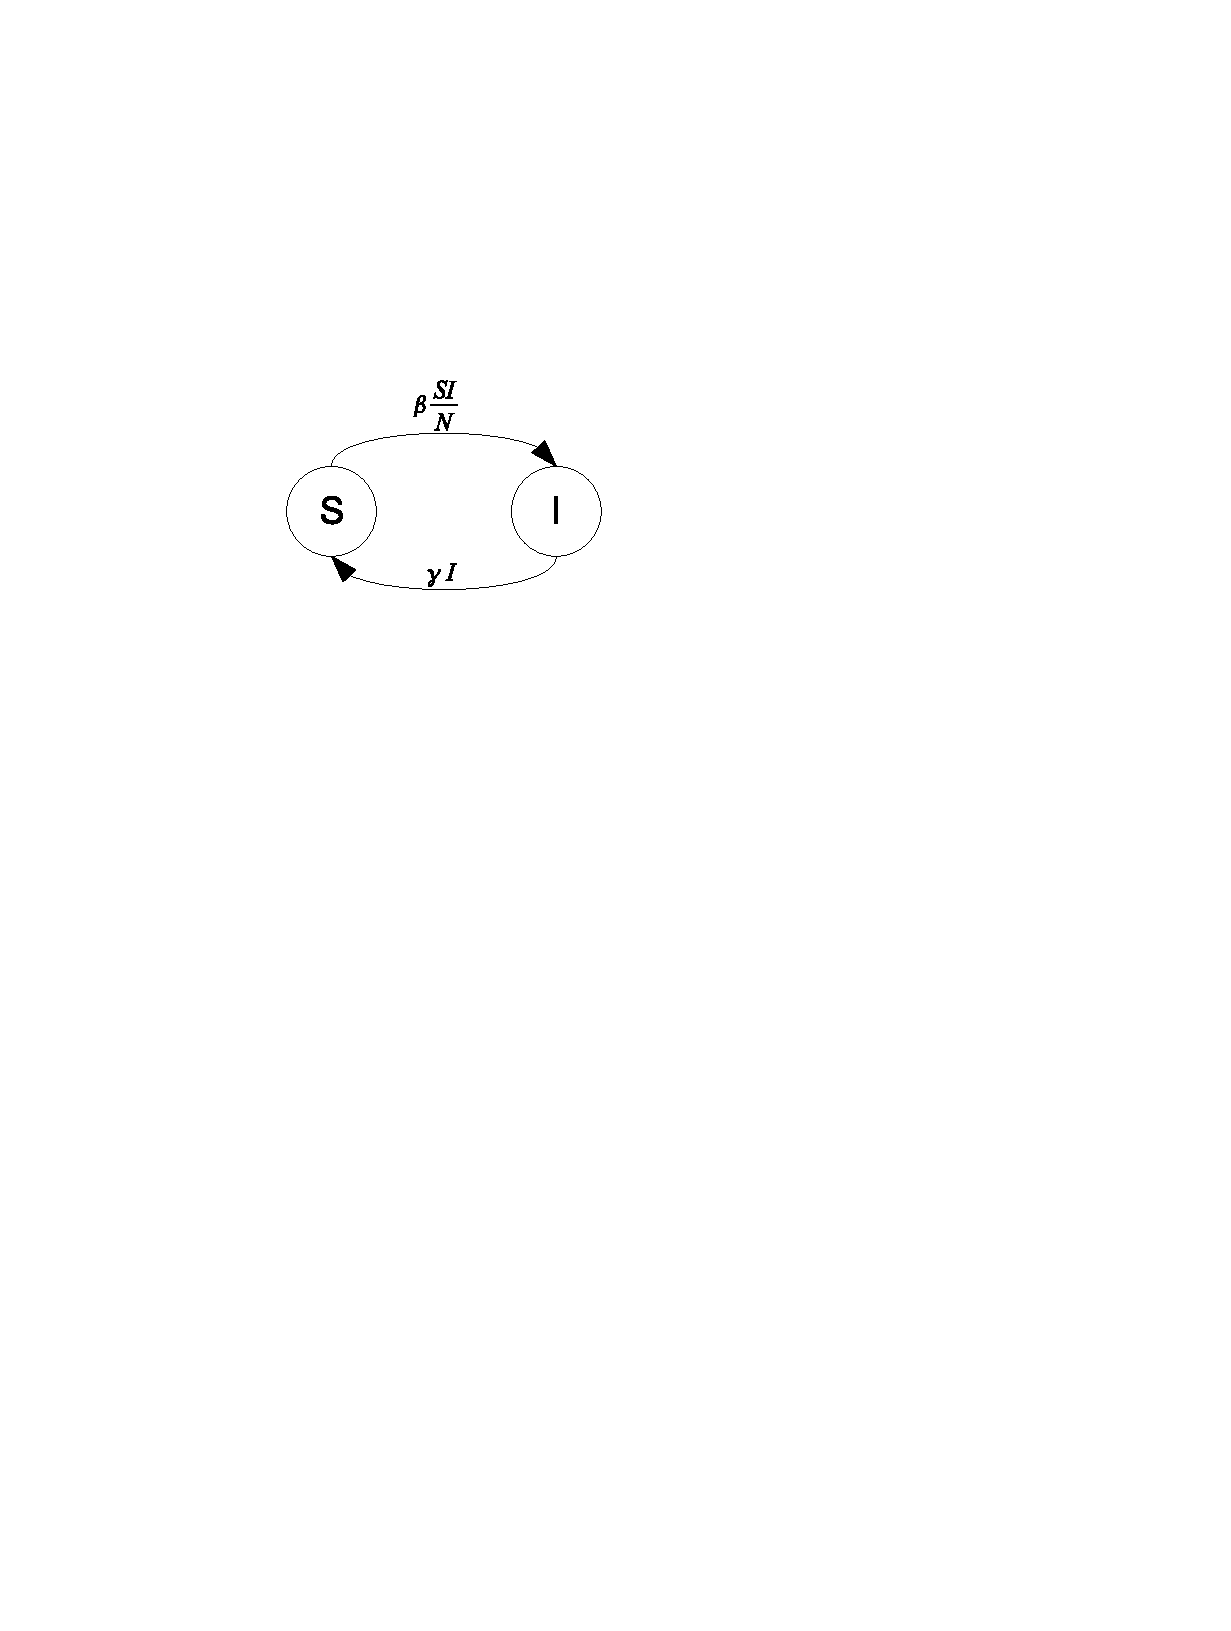
\includegraphics[width=0.5\textwidth]{SIS_nodemography}
\end{center}
}


\frame{
The evolution of $I(t)$ is described by the following equation (see slides on \emph{residence time}):
\[
I'= \beta \frac{(N-I)I}{N}-\gamma I.
\]
Develop and reorder the terms, giving
\begin{equation}\label{sys:I_nodemography}
I'=(\beta-\gamma)I-\frac{\beta}{N} I^2
\end{equation}
This is a logistic-type equation. It can be solved as a Bernoulli equation or as a separable equation, giving, for an initial number of infectives $I(0)=I_0$,
\[
I(t)=\frac{(\beta-\gamma)NI_0}{(\beta-\gamma)Ne^{-(\beta-\gamma)t}+\beta I_0\left(1-e^{-(\beta-\gamma)t}\right)}
\]
}

\frame{
From $S=N-I$, we deduce that the solution $(S(t),I(t))$ for the complete system, with initial condition $S(0)+I(0)=S_0+I_0=N$ is, for $t\geq 0$,
\[
S(t)=N-\frac{(\beta-\gamma)NI_0}{(\beta-\gamma)Ne^{-(\beta-\gamma)t}+\beta I_0\left(1-e^{-(\beta-\gamma)t}\right)}
\]
and 
\[
I(t)=\frac{(\beta-\gamma)NI_0}{(\beta-\gamma)Ne^{-(\beta-\gamma)t}+\beta I_0\left(1-e^{-(\beta-\gamma)t}\right)}
\]
}

\frame{\frametitle{Behavior of the solutions}
Consider only $I$ for the moment.
\[
I(t)=\frac{{\red(\beta-\gamma)}NI_0}{{\red(\beta-\gamma)}Ne^{-{\red(\beta-\gamma)}t}+\beta I_0\left(1-e^{-{\red(\beta-\gamma)}t}\right)}
\]
So
\begin{itemize}
\item If $\beta-\gamma>0$, then $e^{-(\beta-\gamma)t}\to 0$ as $t\to\infty$, and therefore
\[
\lim_{t\to\infty} I(t)=\frac{(\beta-\gamma)NI_0}{\beta I_0}=\frac{\beta-\gamma}{\beta}N=\left(1-\frac{\gamma}{\beta}\right)N.
\]
\item If $\beta-\gamma<0$, then $e^{-(\beta-\gamma)t}\to\infty$ at $t\to\infty$. This implies that the denominator in $I(t)$ tends to $-\infty$ as $t\to\infty$, and so
\[
\lim_{t\to\infty} I(t)=0,\textrm{ with }I(t)>0\textrm{ for all }t.
\]
\item If $\beta=\gamma$, then $I(t)=0$ for all $t$.
\end{itemize}
}

\frame{\frametitle{The basic reproduction number}
Define the \emph{basic reproduction number} (the average number of people that an infectious individual will infect, when introduced in a population of susceptibles) as 
\[
\Rzero=\frac\beta\gamma
\]
We have
\[
\left(\Rzero<1\Leftrightarrow (\beta-\gamma)<0\right)\textrm{ and }\left(\Rzero>1\Leftrightarrow (\beta-\gamma)>0\right).
\]
Therefore, previous cases can be rewritten
\begin{itemize}
\item If $\Rzero<1$, then $\lim_{t\to\infty}I(t)=0$.
\item If $\Rzero>1$, then
\[
lim_{t\to\infty} I(t)=\left(1-\frac{1}{\Rzero}\right)N.
\]
\end{itemize}
(the case $\Rzero=1$ is usually omitted)
}

\frame[containsverbatim]{\frametitle{Plotting this in Maple}
{\tt >} {\red\verb!f:=R->piecewise(R<1,0,R>1,(1-1/R)*1000);!}\\
{\tt >} {\red\verb!plot(f(R),R=0..10);!}
\begin{center}
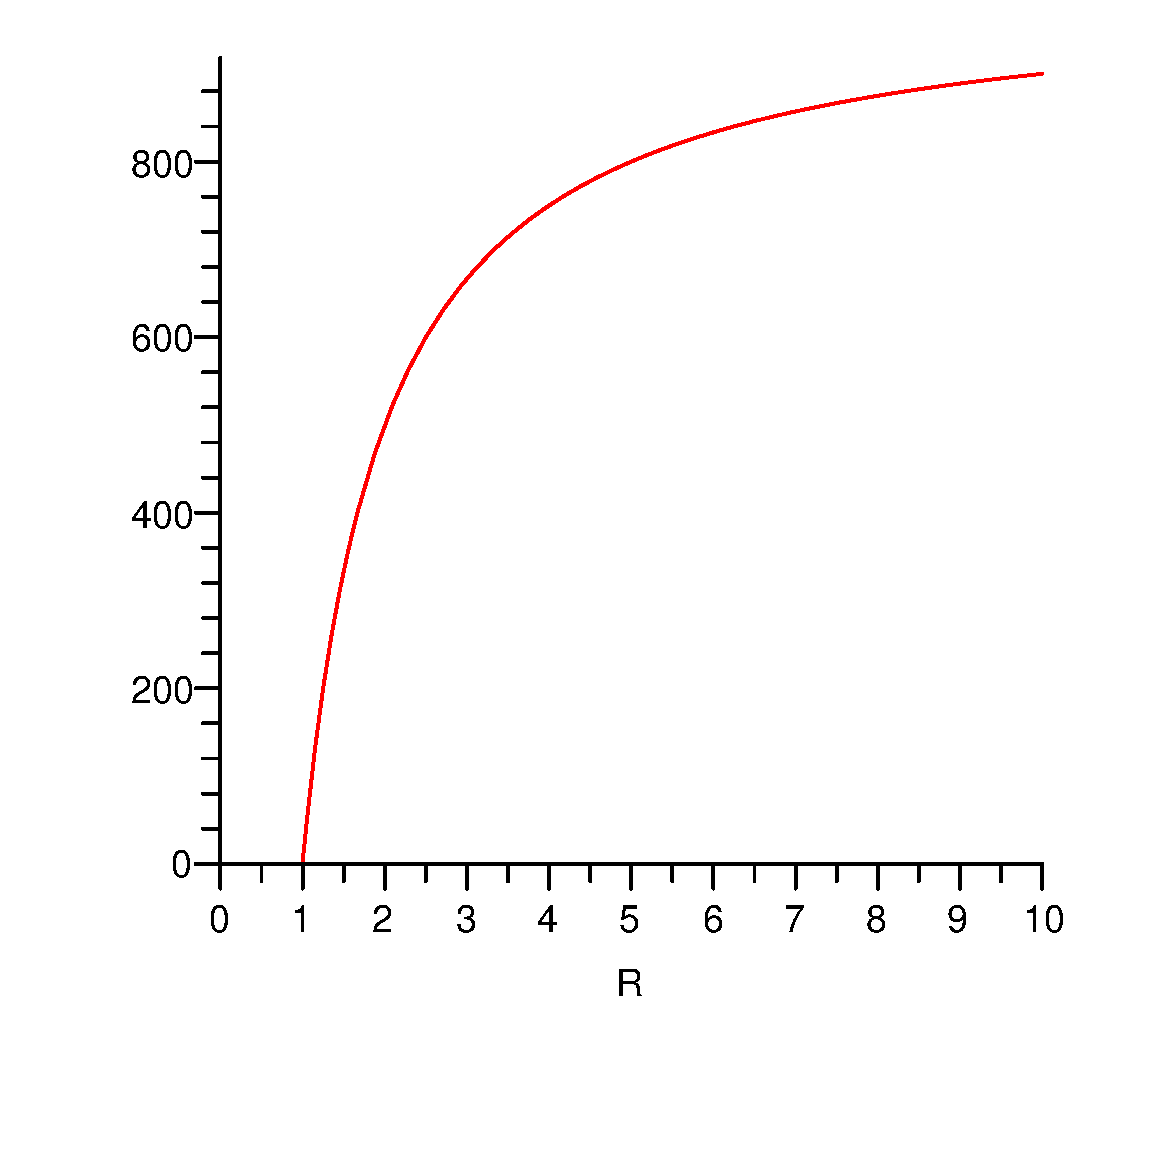
\includegraphics[width=0.6\textwidth]{EEP_fct_R0}
\end{center}
}


\section{SIR model of Kermack and McKendrick}
\frame[plain]{\tableofcontents[current]}

\frame{
\begin{center}
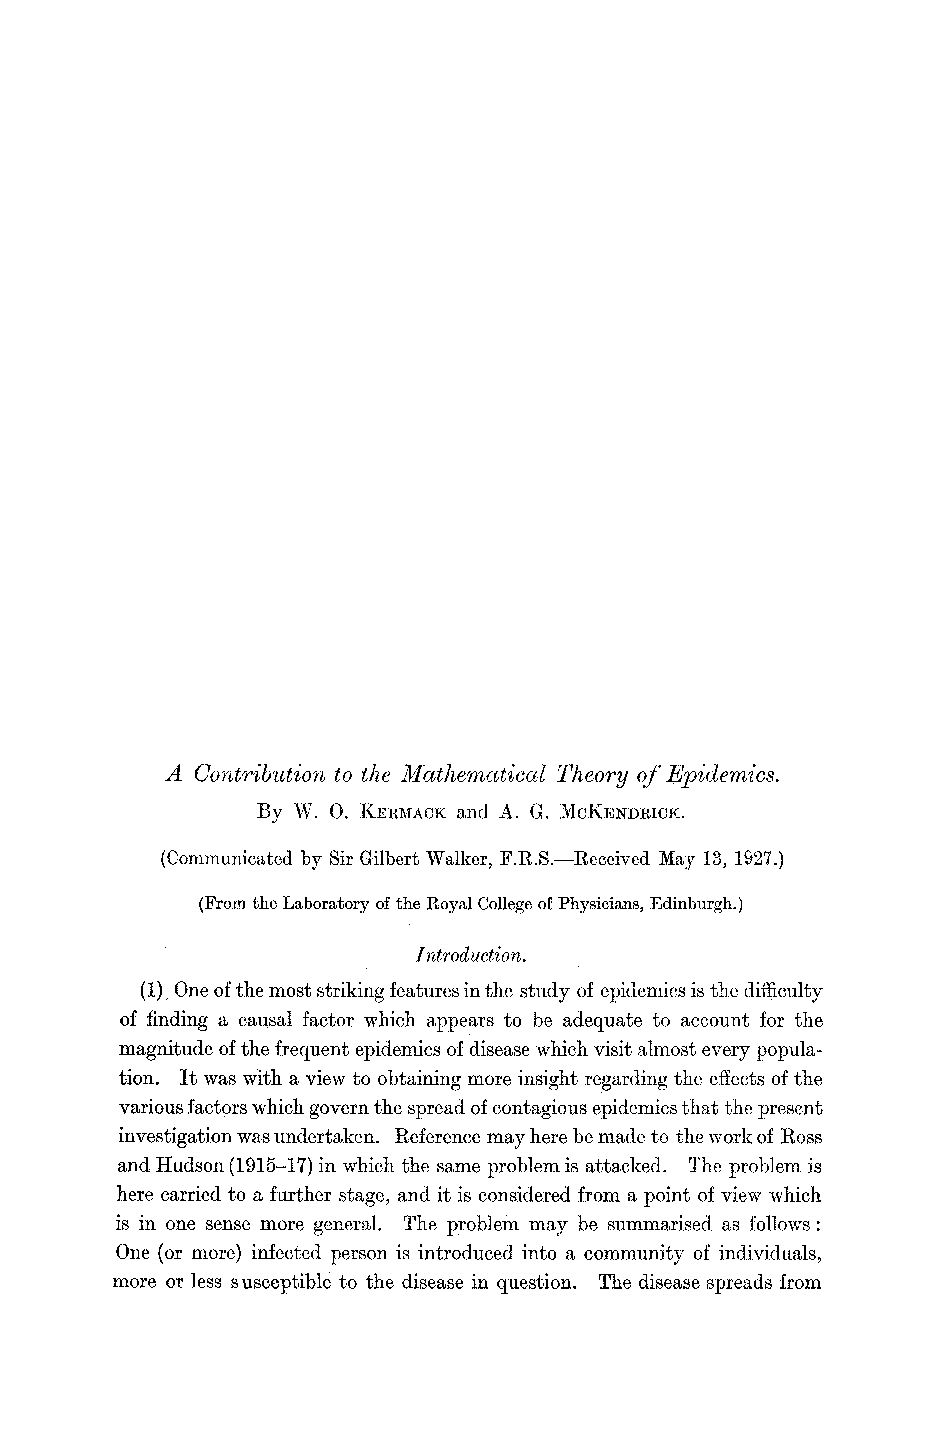
\includegraphics[width=0.9\textwidth]{KMK_title}
\end{center}
}

\frame{
\begin{center}
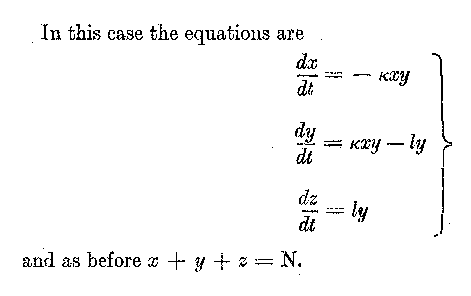
\includegraphics[width=0.7\textwidth]{KMK_model1}
\end{center}
}

\frame{\frametitle{Kermack and McKendrick}
In 1927, Kermack and McKendrick started publishing a series of papers on epidemic models. In the first of their papers, they have this model as a particular case:
\begin{equation}\label{sys:KMK}
\begin{aligned}
S' &= -\beta SI \\
I' &= \beta SI-\gamma I \\
R' &= \gamma I
\end{aligned}
\end{equation}
}

\frame[plain]{
\begin{center}
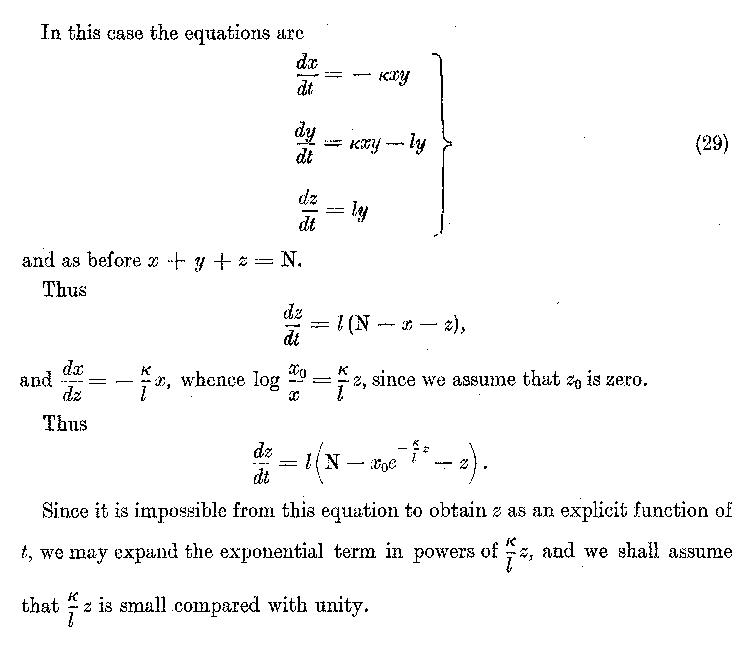
\includegraphics[width=\textwidth]{KMK_model2}
\end{center}
}

\frame{\frametitle{Analyzing the system}
First, note (as KMK) that the total population in the system is constant. This is deduced from the fact that
\[
N'=(S+I+R)'=-\beta SI+\beta SI-\gamma I+\gamma I=0.
\]
Since this is true for all values of $t$, we have $N$ constant.
}

\frame{
Let us ignore the $R$ equation for now.
We can compute
\[
\frac{dI}{dS}=\frac{dI}{dt}\frac{dt}{dS}=\frac{I'}{S'}=\frac{\gamma}{\beta S}-1
\]
This gives
\[
I(S)=S-\frac{\gamma}{\beta}\ln S+K,
\]
which, considering the initial condition $(S_0,I_0)$, is,
\[
I(S)=S-\frac{\gamma}{\beta}\ln S+I_0-(S_0-\frac{\gamma}{\beta}\ln S_0).
\]
This gives a curve in the $(S,I)$ plane.
}


\frame{
\[
I(S)=S-\frac{\gamma}{\beta}\ln S+I_0-(S_0-\frac{\gamma}{\beta}\ln S_0).
\]
Typically, assume $S\approx N$ and $I>0$ small.
Let us denote $S_\infty=\lim_{t\to\infty}S(t)$.

We want to find the value of $S$ when $I\to 0$.
Then
\[
I_0-\frac\gamma\beta\ln S_0=S_\infty -\frac\gamma\beta \ln S_\infty
\]
}

\section{SIRS model with demography}
\frame[plain]{\tableofcontents[current]}

\frame{\frametitle{The SIRS model -- Assumptions (1/2)}
\begin{itemize}
\item Like KMK, individuals are S, I or R.
\item Infection is $\beta SI$ (mass action) or $\beta SI/N$ (proportional incidence).
\item Different interpretation of the R class: R stands for ``recovered'', individuals who are immune to the disease following recovery.
\item Recovery from the disease (movement from I class to R class) occurs at the per capita rate $\gamma$.\\ (Time spent in I before recovery is exponentially distributed.)
\item Immunity can be lost: after some time, R individuals revert back to S individuals.
\item Time spent in R class before loss of immunity is exponentially distributed, with mean $1/\nu$.
\end{itemize}
}

\frame{\frametitle{The SIRS model -- Assumptions (2/2)}
\begin{itemize}
\item There is birth and death of individuals:
\begin{itemize}
\item No vertical transmission of the disease (mother to child) or of immunity, so all birth is into the S class.\\ Birth occurs at the rate $\Pi$.
\item Individuals in all classes die of at the per capita rate $d$, i.e., the average life duration is exponentially distributed with mean $1/d$.
\item The disease is lethal: infected individuals are subject to additional mortality at the per capita rate $\delta$.
\end{itemize}
\end{itemize}
Note that birth and death can have different interpretations:
\begin{itemize}
\item birth and death in the classical sense,
\item but also, entering the susceptible population and leaving it.
\end{itemize}
}

\frame{\frametitle{Flow diagrams for the models}
\begin{description}
\item[Mass action]\qquad
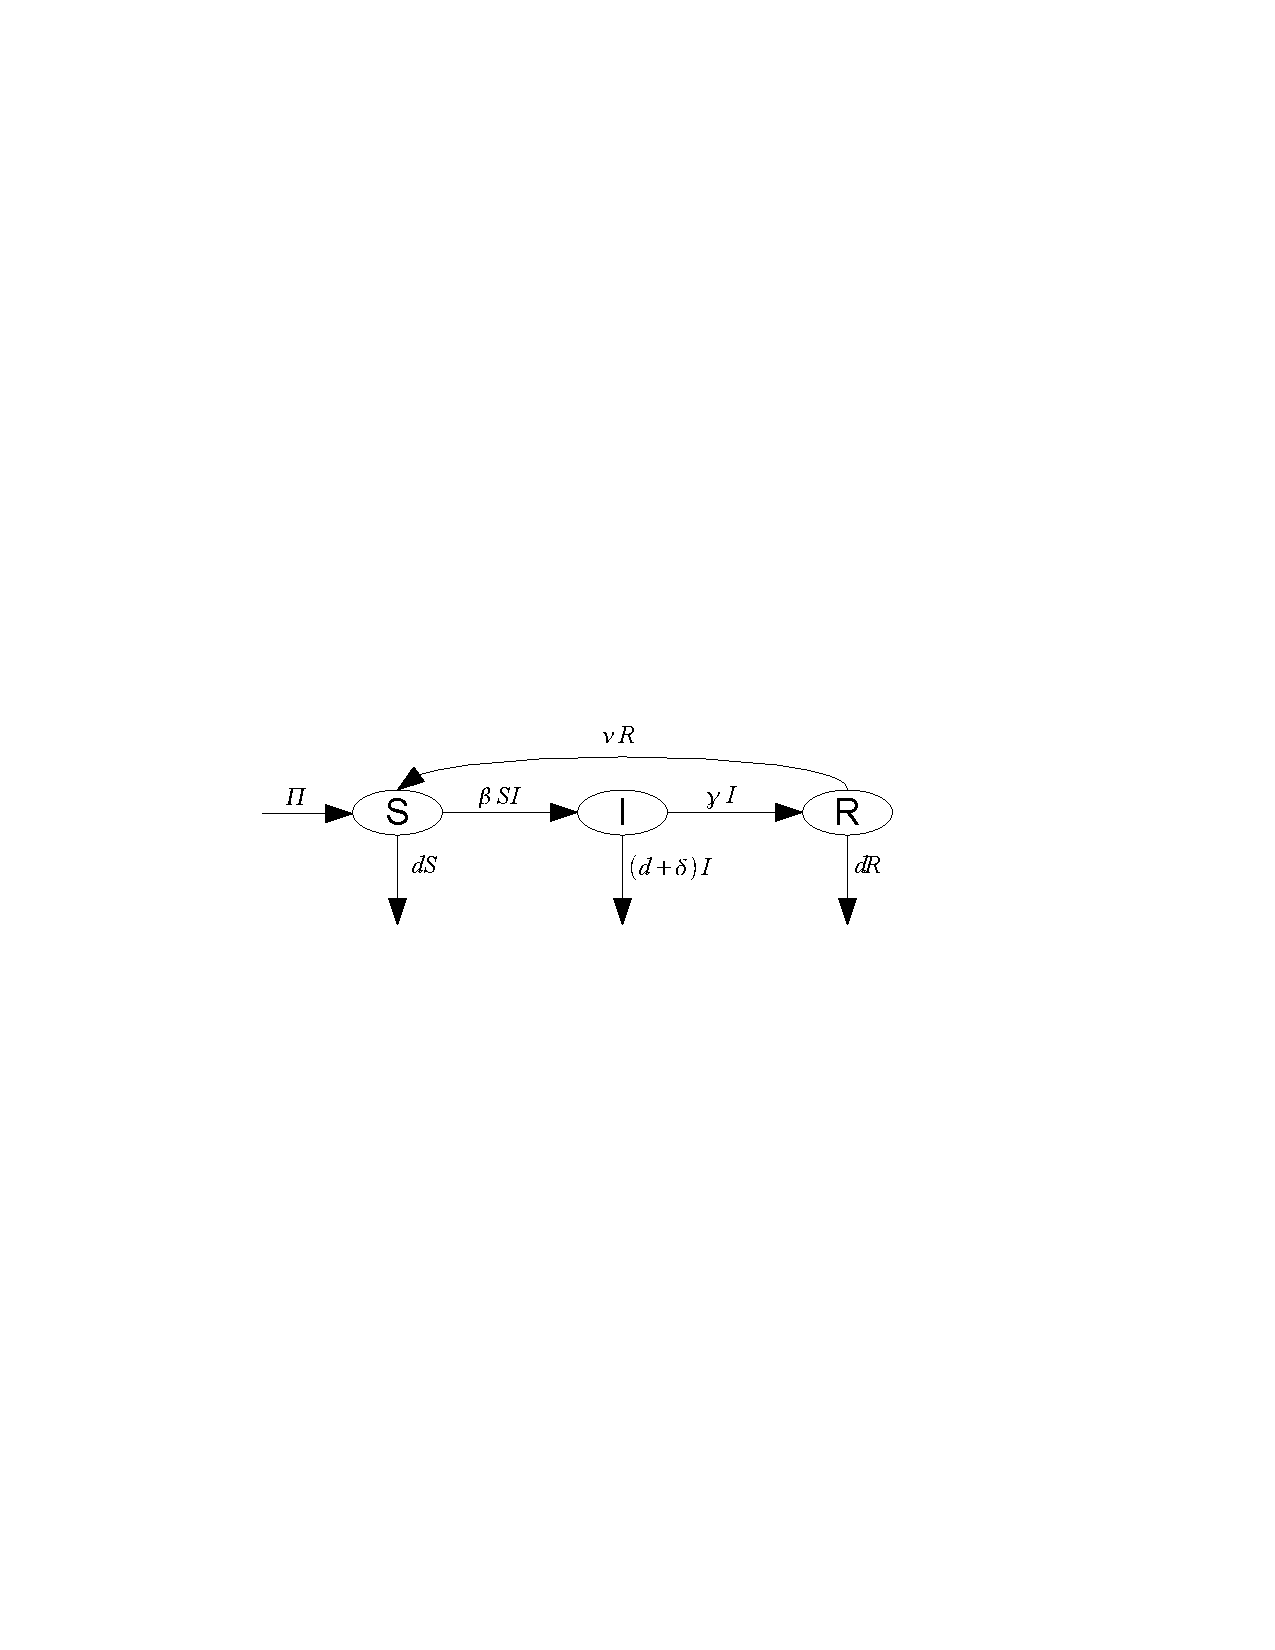
\includegraphics[width=0.75\textwidth]{SIRS_massaction}\vskip1cm
\item[Standard incidence]
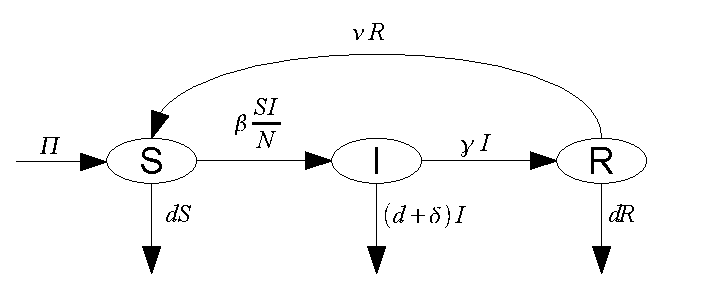
\includegraphics[width=0.75\textwidth]{SIRS_propincidence}
\end{description}
}

\frame{\frametitle{SIRS models}
\begin{description}
\item[Mass action]
\begin{subequations}\label{SIRS_MA}
\begin{align}
S' &= \Pi+\nu R-\beta SI-dS \label{SIRS_MA_S} \\
I' &= \beta SI-(d+\delta+\gamma)I \label{SIRS_MA_I} \\
R' &= \gamma I-(d+\nu)R \label{SIRS_MA_R}
\end{align}
\end{subequations}
\item[Proportional incidence]
\begin{subequations}\label{SIRS_P}
\begin{align}
S' &= \Pi+\nu R-\beta SI-dS \label{SIRS_P_S} \\
I' &= \beta SI-(d+\delta+\gamma)I \label{SIRS_P_I} \\
R' &= \gamma I-(d+\nu)R, \label{SIRS_P_R}
\end{align}
\end{subequations}
where $N=S+I+R$.
\end{description}
}

\frame{\frametitle{SIRS model with mass action incidence}
Consider \eqref{SIRS_MA}:
\begin{align*}
S' &= \Pi+\nu R-\beta SI-dS \\
I' &= \beta SI-(d+\delta+\gamma)I \\
R' &= \gamma I-(d+\nu)R
\end{align*}
}

\frame{\frametitle{Steps of the analysis}
\begin{enumerate}
\item Assess well-posedness of the system:
\begin{enumerate}
\item Determine whether solutions exist and are unique.
\item Determine whether solutions remain in a realistic region and are bounded.
\end{enumerate}
\item Find the equilibria of the system.
\item Determine the local stability properties of the equilibria.
\item Determine the global stability properties of the equilibria ({\bf much harder}, often not possible).
\end{enumerate}
}

\frame{\frametitle{Existence and uniqueness of solutions}
\begin{theorem}[Cauchy-Lipschitz]
Consider the equation $x'=f(x)$, with $x\in\IR^n$, and suppose that $f\in C^1$. Then there exists a unique solution of $x'=f(x)$ such that $x(t_0)=x_0$, where $t_0\in\IR$ and $x_0\in\IR^n$, defined on the largest interval $J\ni t_0$ on which $f\in C^1$.
\end{theorem}
}


\frame{\frametitle{Equilibria}
\begin{definition}[Equilibrium point]
Consider a differential equation
\begin{equation}\label{eq:ODE}
x'=f(x),
\end{equation}
with $x\in\IR^n$ and $f:\IR^n\to\IR^n$.
Then $x^*$ is an equilibrium (solution) of \eqref{eq:ODE} if $f(x^*)=0$.
\end{definition}
}

\frame{\frametitle{Linearization}
Consider $x^*$ an equilibrium of \eqref{eq:ODE}. For simplicity, assume here that $x^*=0$ (it is always possible to do this, by considering $y=x-x^*$).
\vskip1cm
Taylor's theorem:
\[
f(x)=Df(0)x+\frac 12 D^2f(0)(x,x)+\cdots,
\]
where $Df(0)$ is the Jacobian matrix of $f$ evaluated at $0$.
}

\frame{\frametitle{Stability of equilibria}
\begin{definition}[Stable and unstable EP]
Let $\phi_t$ be the flow of \eqref{eq:ODE}, assumed to be defined for all $t\in\IR$. An equilibrium $x^*$ of \eqref{eq:ODE} is (locally) \emph{stable} if for all $\varepsilon>0$, there exists $\delta>0$ such that for all $x\in\mathcal{N}_\delta(x^*)$ and $t\geq 0$, there holds
\[
\phi_t(x)\in\mathcal{N}_\varepsilon(x^*).
\]
The equilibrium point is \emph{unstable} if it is not stable.
\end{definition}
\begin{definition}[Asymptotically stable EP]
Let $\phi_t$ be the flow of \eqref{eq:ODE} is (locally) \emph{asymptotically stable} if there exists $\delta>0$ such that for all $x\in\mathcal{N}_\delta(x^*)$ and $t\geq 0$, there holds
\[
\lim_{t\to\infty}\phi_t(x)=x^*.
\]
\end{definition}
Clearly, Asymtotically Stable $\Rightarrow$ Stable.
}


\frame{\frametitle{Hyperbolic EPs, sinks, sources}
\begin{definition}[Sink]
An equilibrium point $x^*$ of \eqref{eq:ODE} is \emph{hyperbolic} if none of the eigenvalues of the matrix $Df(x^*)$ (Jacobian matrix of $f$ evaluated at $x^*$) have zero real parts.
\end{definition}
\begin{definition}[Sink]
An equilibrium point $x^*$ of \eqref{eq:ODE} is a \emph{sink} if all the eigenvalues of the matrix $Df(x^*)$ have negative real parts.
\end{definition}
\begin{definition}[Source]
An equilibrium point $x^*$ of \eqref{eq:ODE} is a \emph{source} if all the eigenvalues of the matrix $Df(x^*)$ have positive real parts.
\end{definition}
}

\frame{
\begin{theorem}
If $x^*$ is a sink of \eqref{eq:ODE} and for all the eigenvalues $\lambda_j$ of the matrix $Df(x^*)$
\[
\Re(\lambda_j)<-\alpha<0,
\]
where $\Re(\lambda)$ denotes the real part of $\lambda$, then for a given $\varepsilon>0$, there exists $\delta>0$ such that for all $x\in\mathcal{N}_\delta(x^*)$, the flow $\phi_t(x)$ of \eqref{eq:ODE} satisfies
\[
\|\phi_t(x)-x^*\|\leq\varepsilon e^{-\alpha t}
\]
for all $t\geq 0$.
\end{theorem}
\begin{theorem}
If $x^*$ is a stable equilibrium point of \eqref{eq:ODE}, no eigenvalue of $Df(x^*)$ has positive real part.
\end{theorem}
}

\end{document}